% !TEX program = xelatex
% ---------------------------------------------------------------------------
%  Counting the Pentametric areas from an empty square  —  Version 1
%  Compile with:  xelatex counting_areas.tex   (twice)
%  Figures: figs_counting.py    Exact checks: verify_counting.py
% ---------------------------------------------------------------------------
\documentclass[11pt,a4paper]{article}
\usepackage[margin=2.6cm]{geometry}
\renewcommand{\topfraction}{0.9}\renewcommand{\bottomfraction}{0.8}\renewcommand{\textfraction}{0.07}\renewcommand{\floatpagefraction}{0.8}
\usepackage{amsmath,amsthm,mathtools}
\usepackage{fontspec}
\usepackage{unicode-math}
\setmainfont{Latin Modern Roman}
\setmathfont{Latin Modern Math}
\usepackage{graphicx}
\usepackage{enumitem}
\usepackage{xcolor}
\usepackage[hidelinks]{hyperref}
\usepackage{caption}
\usepackage{cite}
\captionsetup{font=small,labelfont=bf}
\theoremstyle{plain}
\newtheorem{theorem}{Theorem}
\newtheorem{proposition}[theorem]{Proposition}
\newtheorem{corollary}[theorem]{Corollary}
\theoremstyle{definition}
\newtheorem{definition}[theorem]{Definition}
\theoremstyle{remark}
\newtheorem{remark}[theorem]{Remark}
\newcommand{\Pa}{\mathfrak{P}}
\newcommand{\leg}[1]{\left(\tfrac{#1}{5}\right)}
\hypersetup{pdftitle={Counting the Pentametric areas from an empty square},pdfauthor={Lluis Garcia Torcal}}

\begin{document}
\begin{center}
{\LARGE Counting the Pentametric areas\\[3pt] from an empty square\par}
\vspace{1em}
{\large Lluis Garcia Torcal\par}
\vspace{0.3em}
{\small Independent researcher, Sabadell, Spain \quad·\quad ORCID \href{https://orcid.org/0009-0007-8570-2536}{0009-0007-8570-2536}\\ \href{mailto:lluisgarciamusic@gmail.com}{lluisgarciamusic@gmail.com}\par}
\vspace{0.3em}
{\small Version 1, October 2026\par}
\end{center}

\begin{abstract}
\noindent The Pentametric areas $\Pa(n)=\bigl(n^2+4\leg{n}\bigr)/5$ are usually written as a value plus a correction of $\pm4/5$. Here we read every quantity as a \emph{count}. Starting from an empty square, the classical lines from each corner to the midpoint of a far side give a square of area $1/5$, the circle of origins and the two lines of Holden (1975) through the centres of the Fibonacci squares, with no grid drawn in advance. Counted in cells of the grid they define (area $1/10$), the square of side $n$ has the area of $10n^2$ cells and the Pentametric square that of $2\bigl(n^2+4\leg{n}\bigr)$ cells; the correction is the blue square of the $2\times2$ square, $2^2/5$, added or taken away. Along Holden's lines, every Fibonacci square begins and ends at a whole number of thirds of the origins unit, $2L_{k-2}$ and $2L_{k+2}$. Finally, when the square of side $n$ is split into $n\times n$ unit squares, its scaled origin lands exactly on an origin of one of them, or exactly on a corner when $5\mid n$: which one is decided by $n\bmod 5$, its sign by the Legendre symbol, and at the Lucas numbers it turns one quarter turn per Fibonacci square, at the same rate as the centres in Holden's tiling, though in the opposite sense. All statements are elementary and checked in exact arithmetic.
\end{abstract}

\section{Introduction}
In earlier notes \cite{gt,rhombus,origins} we met the origins unit $\rho=\sqrt{0.1}$, the circle of origins of radius $\rho$ about the centre $O$ of the unit square, and its eight origins $(\pm\tfrac3{10},\pm\tfrac1{10})$, $(\pm\tfrac1{10},\pm\tfrac3{10})$. The Pentametric areas
\[
\Pa(n)=\frac{n^2+4\leg{n}}{5}=\frac{n^2}{5}\pm\frac45\quad(\text{or }n^2/5\text{ when }5\mid n)
\]
are whole numbers, and $\Pa(L_k)=F_k^2$ at the Lucas numbers \cite{gt}. The aim of this note is to show these areas, and the geometry around them, as \emph{counts}: of cells, of thirds of $\rho$, and of quarter turns, rather than as a value plus a correction. Throughout, the frame is the unit square centred at $O=(0,0)$; $\leg{n}$ is the Legendre symbol ($0$ if $5\mid n$, $+1$ if $n\equiv\pm1$, $-1$ if $n\equiv\pm2 \pmod 5$), which we also call the \emph{breath} of $n$.

\section{From an empty square}
\begin{proposition}[the classical $1/5$ square]\label{prop:empty}
In the unit square, draw from each corner the line to the midpoint of the second side met when going anticlockwise round the square (the line from $(-\tfrac12,-\tfrac12)$ to $(\tfrac12,0)$ and its images under quarter turns about $O$). These four lines meet at right angles in the four points $(-\tfrac1{10},-\tfrac3{10})$, $(\tfrac3{10},-\tfrac1{10})$, $(\tfrac1{10},\tfrac3{10})$, $(-\tfrac3{10},\tfrac1{10})$: the corners of a square of side $\sqrt{0.2}$ and area $1/5$. The circle through them is the circle of origins. The mirror construction gives the other four origins.
\end{proposition}
\begin{proof}
For example, the line from $(-\tfrac12,-\tfrac12)$ to $(\tfrac12,0)$ is $y=\tfrac{x}{2}-\tfrac14$, and the line from $(-\tfrac12,\tfrac12)$ to $(0,-\tfrac12)$ is $y=-2x-\tfrac12$; they meet at $x=-\tfrac1{10}$, $y=-\tfrac3{10}$, at right angles (slopes $\tfrac12$ and $-2$). The other corners follow by quarter turns about $O$, and $(\tfrac1{10})^2+(\tfrac3{10})^2=\rho^2$.
\end{proof}
This square is the classical puzzle of cutting a square into five equal squares, much older than the book in which we found it: a Spanish book of recreations (1954; 4th ed.\ 1957) \cite{claraso}, where the central piece is exactly this square, turned the same way. What is new here is only the reading of its corners. At the origin $H=(\tfrac3{10},-\tfrac1{10})$ the tangent of the circle of origins is the line $3x-y=1$, and the perpendicular is $x+3y=0$, through $O$. Fix the Fibonacci tiling with square $1$ the unit square, square $2$ below it (centre $(0,-1)$), square $3$ to the right, and so on, turning anticlockwise. Then these are its even and odd lines in the sense of Holden \cite{holden} and Gardiner \cite{gardiner}: the centres of the even squares lie on $3x-y=1$ and those of the odd squares on $x+3y=0$, the centre $C_k$ at $L_k$ origins units from $H$ (Fig.~\ref{fig:empty}; see \cite{origins} for the uniqueness of this circle). So Holden's two lines can be drawn with a ruler alone from an empty square (the midpoints of the sides can themselves be found with a ruler, from the diagonals and the parallel sides): the odd line is $OH$, and the even line joins $H$ to the corner $(\tfrac12,\tfrac12)$.

\begin{figure}[ht]
\centering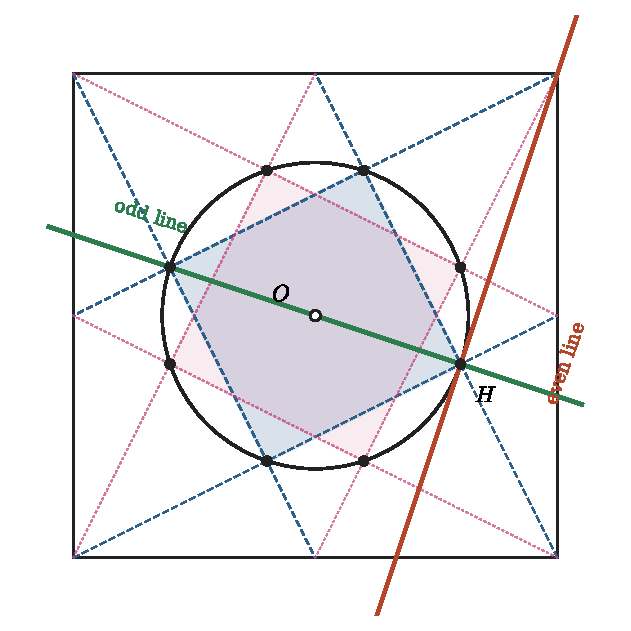
\includegraphics[width=0.48\textwidth]{fig1_empty_square.pdf}
\caption{From an empty square. The blue dashed lines (corner to the midpoint of a far side) cross at the corners of the blue square of area $1/5$; the pink lines give its mirror. The circle through them is the circle of origins. At the origin $H$, its tangent is the even line and its perpendicular, through $O$, the odd line.}
\label{fig:empty}
\end{figure}

\section{Counting cells and thirds}
The lines $3x-y\in\mathbb Z$ and $x+3y\in\mathbb Z$, the \emph{origins grid}, cut the plane into square cells of side $\rho$ and area $1/10$. Along a side of the unit square one family crosses every $1/3$ and the other every $1$: a side is ``$3$ one way and $1$ the other'', and $3^2+1^2=10$.
\begin{proposition}[cells]\label{prop:cells}
The square of side $n$ has the area of $10n^2$ cells (its sides are not grid lines, so this is a count by area); its circle of origins (radius $n\rho$) has area $n^2$ times $\pi/10$. The blue square is made of exactly $2$ cells (four half-cells: its side is the diagonal of one cell, and its corners and $O$ are grid points), and scaled by $n$ it has the area of $2n^2$ cells. The Pentametric square of area $\Pa(n)$ has the area of
\[
10\,\Pa(n)=2n^2+8\leg{n}\ \text{cells},
\]
always a whole number: the blue square scaled by $n$, with $8$ cells added, taken away, or neither.
\end{proposition}
The $8$ cells are themselves a square we already know: the blue square of the $2\times2$ square, of area $2^2/5=4/5$. So
\[
\boxed{\ \Pa(n)=\frac{n^2}{5}+\leg{n}\frac{2^2}{5}\ }
\]
is the blue square of $n$ plus or minus the blue square of $2$ (Fig.~\ref{fig:breath}). Inside the circle of origins, the crossings of the blue and pink squares are the corners of two smaller squares, of areas $1/8$ and $1/9$ \cite{origins}; the first is turned by $45^\circ$ (corners $(\pm\tfrac14,0)$, $(0,\pm\tfrac14)$), the second is upright (corners $(\pm\tfrac16,\pm\tfrac16)$) and, of side $1/3$ of the side of the unit square, tiles it exactly nine times: the grid of thirds of the side, on whose lines lie the vertices $A$ and $C$ of the Epitetartic Rhombus \cite{rhombus}. The ``$4$'' of the formula is $2^2$; this is also why $\Pa(2)=0$: at $n=2$ the breath takes away the square's own blue square.

\begin{figure}[ht]
\centering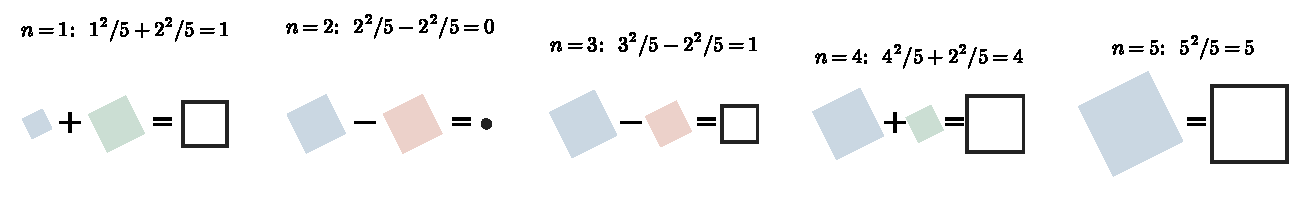
\includegraphics[width=\textwidth]{fig2_breath.pdf}
\caption{The breath as a square. For $n=1,\dots,5$: the blue square of the square of side $n$ (area $n^2/5$), plus (green) or minus (red) the blue square of the $2\times2$ square (area $2^2/5$), gives the Pentametric square $\Pa(n)$ (black, drawn upright). At $n=5$ there is no breath.}
\label{fig:breath}
\end{figure}

Along Holden's lines the natural ruler is a \emph{third} of $\rho$: a piece of one of these lines is $\sqrt{10}/3$ times its longer projection on the axes, since the lines have slope $\pm3$ or $\pm\tfrac13$, so $1/5$ of a side along an axis becomes $\tfrac23\rho$ along the line. In the unit square the four arms from $H$ to the sides are $2,4,6,8$ thirds of $\rho$, and each line crosses the square in $10$ thirds; the diagonals of the Epitetartic Rhombus \cite{rhombus} are $10$ and $8$ thirds (in the square of side $n$: $10n$ and $8n$).
\begin{proposition}[thirds]\label{prop:thirds}
Let $C_k$ be the centre of the $k$-th Fibonacci square (side $F_k$), on its Holden line (the odd line for odd $k$, the even line for even $k$) at $L_k$ origins units from the crossing $H$ \cite{holden}. Measure distances along that line from $H$, positive towards $C_k$, and put $L_{-1}=-1$. Then the square is entered and left at
\[
2L_{k-2}\quad\text{and}\quad 2L_{k+2}\quad\text{thirds of }\rho
\]
($k=1$: $-2$ and $8$, so $H$ lies inside the square; $k=2$: $4$ and $14$; $k=3$: $2$ and $22$; $k=4$: $6$ and $36$; \dots).
\end{proposition}
\begin{proof}
The line passes through the centre with slope $\pm3$ or $\pm\tfrac13$, so it meets two opposite sides of the square, and the half-chord is $\tfrac{F_k}{2}\cdot\tfrac{\sqrt{10}}{3}=\tfrac{5F_k}{3}\rho$. So the ends are at $\tfrac{3L_k\pm5F_k}{3}\rho$, and $3L_k\pm5F_k=2L_{k\pm2}$, because $L_{k+2}+L_{k-2}=3L_k$ and $L_{k+2}-L_{k-2}=5F_k$.
\end{proof}

\section{Where the origin lands}
Split the square of side $n$, centred at $O$, into $n\times n$ unit squares. Their centres are the points of $\mathbb Z^2$ if $n$ is odd and of $(\tfrac12,\tfrac12)+\mathbb Z^2$ if $n$ is even. Scale the origin $z=H=(\tfrac3{10},-\tfrac1{10})$, the crossing of Holden's lines, by $n$, and compare $nz$ with the centre $c$ of the unit square it falls in. We identify points with complex numbers, so $z=(3-i)/10$ and multiplication by $i^{-1}$ is a quarter turn clockwise.
\begin{theorem}[landing]\label{thm:landing}
For every $n\ge1$:
\begin{enumerate}[label=(\alph*),nosep]
\item if $5\nmid n$, the point $nz$ is exactly an origin of the unit square it falls in: $nz-c=i^{-t}z$ (turned by $t$ quarter turns clockwise), with $t=0,1,2,3$ for $n\equiv1,3,4,2\pmod5$;
\item if $5\mid n$, the point $nz$ is exactly a corner of the unit squares.
\end{enumerate}
\end{theorem}
\begin{proof}
For $n=1,\dots,5$ one checks directly: $z$; $2z=(\tfrac12,-\tfrac12)+(\tfrac1{10},\tfrac3{10})$; $3z=(1,0)+(-\tfrac1{10},-\tfrac3{10})$; $4z=(\tfrac32,-\tfrac12)+(-\tfrac3{10},\tfrac1{10})$; $5z=(\tfrac32,-\tfrac12)$, a corner. Going from $n$ to $n+5$ adds $5z=(\tfrac32,-\tfrac12)\in(\tfrac12,\tfrac12)+\mathbb Z^2$, which carries the centres for $n$ onto the centres for $n+5$ (the parity of $n$ changes). So the offset $nz-c$ depends only on $n\bmod5$. When $5\nmid n$ both coordinates of the offset are at most $\tfrac3{10}<\tfrac12$ in size, so $nz$ lies inside exactly one unit square and $c$ is the nearest centre; when $5\mid n$, $nz$ is a corner shared by four unit squares.
\end{proof}
The landing origin always belongs to the same family, the blue square. The two origins half a turn apart ($t=0,2$) lie on the line through the centre of that unit square parallel to the odd line, the direction of the odd Fibonacci squares; the quarter-turned ones ($t=1,3$) lie on the perpendicular, parallel to the even line, the direction of the even squares; and the multiples of $5$ land on a corner (Fig.~\ref{fig:landing}).

\begin{corollary}[the breath from the landing]\label{cor:sign}
If $5\nmid n$ and $d=nz-c$, then
\[
100\bigl[(d\cdot z)^2-(d\times z)^2\bigr]=\leg{n},
\]
using only products and squares. If $5\mid n$, then $|d|^2=\tfrac12$ instead of $\tfrac1{10}$, whichever of the four neighbouring centres is taken: the rest.
\end{corollary}
\begin{proof}
With $d=i^{-t}z$, $d\cdot z=\tfrac1{10}\cos\tfrac{t\pi}2$ and $d\times z=\pm\tfrac1{10}\sin\tfrac{t\pi}2$, so the bracket is $\tfrac1{100}\cos t\pi=\tfrac1{100}(-1)^t$; and $t$ is even exactly when $n\equiv\pm1$.
\end{proof}

\begin{corollary}[a quarter turn per Fibonacci square]\label{cor:holden}
At the Lucas numbers, $t(L_k)=k-1\pmod 4$: the landing turns one quarter turn from each Fibonacci square to the next, at the same rate as the centres of the Fibonacci squares in Holden's tiling \cite{holden,gardiner} (here clockwise, while the tiling turns anticlockwise). No Lucas number is a multiple of $5$, so only the two breaths $\pm1$ occur there, alternating with $k$.
\end{corollary}
\begin{proof}
$L_1=1$, $L_2=3$ and $3^2\equiv3+1\pmod5$, so $L_k\equiv3^{k-1}\pmod 5$ for $k\ge1$; the order $1,3,4,2$ of Theorem~\ref{thm:landing} is $3^0,3^1,3^2,3^3$.
\end{proof}

\begin{figure}[ht]
\centering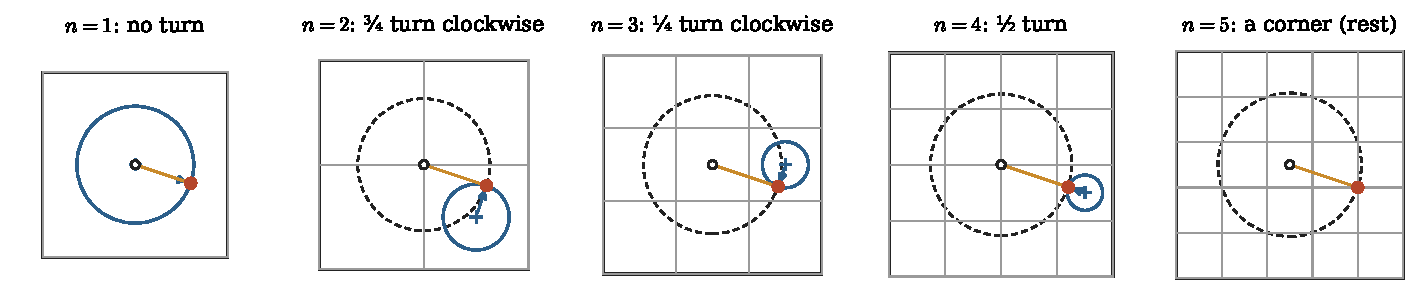
\includegraphics[width=\textwidth]{fig3_landing.pdf}
\caption{Where the origin lands, $n=1,\dots,5$. The square of side $n$ is split into unit squares; the dashed circle is its circle of origins (radius $n\rho$), and the red point the scaled origin $nz$. It falls exactly on an origin of a unit square (blue circle, arrow from that square's centre), turned $0$, $\tfrac34$, $\tfrac14$, $\tfrac12$ of a turn clockwise; at $n=5$ it falls on a corner.}
\label{fig:landing}
\end{figure}

As a consistency check, Corollary~\ref{cor:sign} agrees, for every $n\le5778$, with the sign of $\Pa(n)-n^2/5$ in the author's spreadsheet of the Pentametric areas. The arithmetic behind it is classical: $10z=3-i$ in the Gaussian integers, $3^2+1^2=10$, and $5=(2+i)(2-i)$ \cite{ir}. We have not found this geometric reading in the sources we consulted \cite{holden,hoggatt,gardiner}.

\section{Mirror squares}
Reflect the unit square in its right side, $x=\tfrac12$. The two squares share the side $x=\tfrac12$, and in particular the corner $F=(\tfrac12,-\tfrac12)$, and the crossings $H=(\tfrac3{10},-\tfrac1{10})$ and $H'=(\tfrac7{10},-\tfrac1{10})$ are mirror images.
\begin{proposition}\label{prop:mirror}
\begin{enumerate}[label=(\alph*),nosep]
\item The circle about $H$ through $F$ (radius $\sqrt2\rho$) passes through the origins $\pm(\tfrac1{10},\tfrac3{10})$ of the first square's circle of origins and through the origin $(\tfrac7{10},\tfrac1{10})$ of the mirror square. These four points are the corners of a square centred at $H$, of area $2/5$ ($4$ cells), with sides along Holden's directions; likewise for $H'$.
\item The odd line $x+3y=0$ of the first square is tangent to the circle of origins of the mirror square, at its origin $(\tfrac9{10},-\tfrac3{10})$; and symmetrically.
\end{enumerate}
\end{proposition}
\begin{proof}
(a) Each of the four points is at squared distance $\tfrac15$ from $H$, and their differences are $(\pm\tfrac35,\mp\tfrac15)$ and $(\mp\tfrac15,\mp\tfrac35)$, of squared length $\tfrac25$. (b) The distance from $(1,0)$ to $x+3y=0$ is $1/\sqrt{10}=\rho$, and the foot of the perpendicular is $(\tfrac9{10},-\tfrac3{10})$.
\end{proof}

\begin{figure}[ht]
\centering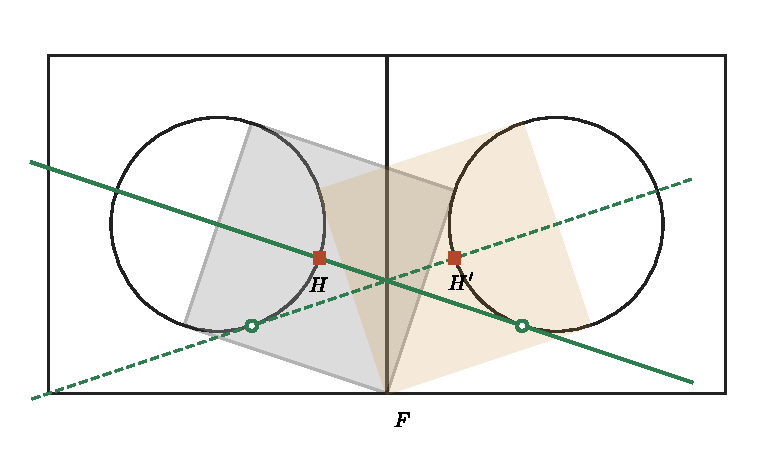
\includegraphics[width=0.62\textwidth]{fig4_mirror.pdf}
\caption{A unit square and its mirror. Grey: the square of area $2/5$ centred on the crossing $H$, with corners $F$, two origins of its own circle and one of the mirror circle; gold: its mirror, centred on $H'$. Each odd line (solid, dashed) is tangent to the neighbour's circle of origins at an origin (open dots).}
\label{fig:mirror}
\end{figure}

\section{Remarks}
\begin{remark}[interpretation]
The breath can be read as a rhythm, \emph{expand} ($+1$), \emph{contract} ($-1$), \emph{rest} ($0$), in the order $0,+,-,-,+$ along $n$. Theorem~\ref{thm:landing} shows it as a place: the scaled origin either keeps to the direction of the odd line, turns to the direction of the even line, or rests on a corner.
\end{remark}
\begin{remark}[interpretation]
The author's working view is that nature only adds and subtracts; multiplication and division are faster ways of repeating them, and squares and square roots are the geometric proportions of numbers (a square, and the units inside it). The landing needs nothing but these: at each step one adds $z=(\tfrac3{10},-\tfrac1{10})$ and subtracts back to the nearest centre, and the breath $0,+1,-1,-1,+1$ appears by itself, with no table of cases; Corollary~\ref{cor:sign} reads its sign with products and squares only.
\end{remark}

\section*{Credits and references}
Holden's lines are due to Holden \cite{holden}, with the generalisation by Hoggatt and Alladi \cite{hoggatt} and the coordinates of Gardiner \cite{gardiner}. The $1/5$ square is a classical recreation \cite{claraso}. The scripts \texttt{verify\_counting.py} and \texttt{figs\_counting.py} and the GeoGebra files are supplied with this note.

\paragraph{Acknowledgements and use of AI.} The construction from an empty square, the reading of the classical $1/5$ square as the source of the origins, the counting in cells and thirds, the mirror squares and the idea of splitting a square into unit squares as quarters of a bigger one are the author's, found in GeoGebra and in his spreadsheets of the Pentametric areas. Claude (Anthropic, Opus 5.5) was used to verify the statements in exact arithmetic, to put the landing rule and its proofs in algebraic form, to prepare the figures and to help draft the text; the author checked and approved every statement. Licence: CC BY 4.0 for this note, MIT for the Python scripts.

\begin{thebibliography}{9}\small
\bibitem{claraso} N. Clarasó, \emph{Enciclopedia de la simpatía}, 4th ed., Gassó Hnos.\ (Osa Menor), Barcelona, 1957 (1st ed.\ 1954), pp.~172--173 (section ``Alardes de geometría amena'': ``Dividir un cuadrado en cinco cuadrados iguales'', figs.~79--80).
\bibitem{gt} L. Garcia Torcal, \emph{The Pentametric Cycle: A Nested Palindrome Encoding the Pythagorean Consonances}, preprint, Zenodo (2026), \href{https://doi.org/10.5281/zenodo.23183108}{doi:10.5281/zenodo.23183108}.
\bibitem{rhombus} L. Garcia Torcal, \emph{The Epitetartic Rhombus}, note, Zenodo (2026), \href{https://doi.org/10.5281/zenodo.23325442}{doi:10.5281/zenodo.23325442}.
\bibitem{origins} L. Garcia Torcal, \emph{The Origin of Origins}, note, Zenodo (2026), \href{https://doi.org/10.5281/zenodo.23486276}{doi:10.5281/zenodo.23486276}.
\bibitem{gardiner} T. Gardiner, 68.15 The Fibonacci spiral, \emph{The Mathematical Gazette} \textbf{68} (1984) 120.
\bibitem{hoggatt} V.~E. Hoggatt, Jr. and K. Alladi, Generalized Fibonacci tiling, \emph{The Fibonacci Quarterly} \textbf{13} (1975) 137--144.
\bibitem{holden} H.~L. Holden, Fibonacci tiles, \emph{The Fibonacci Quarterly} \textbf{13} (1975) 45--49.
\bibitem{ir} K. Ireland and M. Rosen, \emph{A Classical Introduction to Modern Number Theory}, 2nd ed., Springer, 1990.
\end{thebibliography}
\end{document}
